% June 2015 (TOC contents linked in blue in pdf file)
%This template was prepared by Dorothea F. Brosius of the 
%Institute for Electronics and Applied Physics, University of Maryland, College Park, MD
%The template was last updated in June 2015
%Thesis Main Page used with thesis.sty based on the
%University of Maryland Electronic Thesis and Dissertation (ETD) Style Guide (2014)

%The YourInformation file was created by Freja Nordsiek, 2014.
%Code for linking the TOC titles to the text in the pdf file was created by Freja Nordsiek, 2014.


% Select the version that fits how you are making this LaTeX document (its driver).
% The first two are the most likely ones to be needed.
%
\newcommand{\mydriver}{pdftex} %Making a PDF directly using pdflatex.
%\newcommand{\mydriver}{dvipdfmx} %Making a DVI and converting that to PDF using dvipdfmx.
% \newcommand{\mydriver}{dvipdfm} %Making a DVI and converting that to PDF using dvipdfm.
% \newcommand{\mydriver}{dvips} %Making a DVI and converting that to PS using dvips (may later be converted to PDF).  (Used with my pc)
% \newcommand{\mydriver}{dvipsone} %Making a DVI and converting that to PS using dvipsone (may later be converted to PDF).
% \newcommand{\mydriver}{ps2pdf} %Same as the one for dvips except it is compatible with Ghostscript's PDF writer.


\documentclass[12pt,\mydriver]{thesis}  %12pt is larger than 11pt

\usepackage{titlesec}
   \titleformat{\chapter}
      {\normalfont\large}{Chapter \thechapter:}{1em}{}

\usepackage{graphicx}
\usepackage{epstopdf}
\epstopdfsetup{update} % only regenerate pdf files when eps file is newer
\usepackage{cite}
\usepackage{lscape}
\usepackage{indentfirst}
\usepackage{latexsym}
%\usepackage{amsmath}
\usepackage{multirow}
\usepackage{tabls}
\usepackage{wrapfig}
\usepackage{slashbox}
\usepackage{longtable}
\usepackage{supertabular}
\usepackage{subfig} % make it possible to include more than one captioned figure/table in a single float
\usepackage{subeqn}
%\usepackage{subfigure}
\usepackage[pdftex, bookmarks, colorlinks=true, plainpages=false, citecolor=blue, urlcolor=blue, filecolor=blue, linkcolor=blue]{hyperref} 
	%Works with PcTex.  You may have to choose one of the drivers above if dvips does not work.

\newcommand{\tbsp}{\rule{0pt}{18pt}} %used to get a vertical distance after \hline
\renewcommand{\baselinestretch}{2}
\setlength{\textwidth}{5.9in}
\setlength{\textheight}{9in}
\setlength{\topmargin}{-.50in}
%\setlength{\topmargin}{0in}    %use this setting if the printer makes the the top margin 1/2 inch instead of 1 inch
\setlength{\oddsidemargin}{.55in}
\setlength{\parindent}{.4in}


\begin{document}

\pagestyle{plain}
\pagenumbering{roman}
\setcounter{page}{2}

\setlength{\parskip}{0em}
\renewcommand{\baselinestretch}{2}
\small\normalsize

%Pages from this point start at Arabic numeral 1
\setcounter{page}{1}
\pagenumbering{arabic}
%Chapter 6


%todo:
% Look up old "best" steering solution
% re-plot old "best steering" solution 
% Get umer steering diagram from laptop
% Vertical steering SSV run
% WRite up simulated annealing
% 

\renewcommand{\thechapter}{6}

\chapter{Steering and Orbit Correction}
\label{ch:steering}

\section{Motivation}

Precise control of centroid orbit is necessary for good beam recirculation, with low losses due to large centroid deviations. This allows for observation of beam losses due to more complex effects, such as resonant excitation of particle and/or beam envelope amplitudes, as well as longitudinal losses. 
The proposed quasi-integrable nonlinear optics experiment has, as its lowest-order, most straightforward diagnostic, a characterization of resonantly driven beam losses with and without nonlinear damping. Therefore, a reduction of transverse scraping losses is imperative for observation of these likely slower loss rates. Additionally, the nonlinear optics experiments require a low-current, high-emittance $60 \mu A$ beam. A large emittance beam corresponds to a large cross-section beam in configuration space, which places a more stringent requirement on steering tolerances. %todo: link to table of UMER beam quantities

In an ideal linear accelerator, there exists a "reference trajectory," which describes the path of an ideal particle. This trajectory is typically centered within the focusing quadrupoles and the beam pipe. A beam with imperfect injection conditions will oscillate about the ideal trajectory. 
In this section, we define "first-turn orbit" to mean the measured or simulated centroid trajectory on the first turn. "Closed orbit" refers to the orbit about which the trajectory oscillates. This is also referred to as the "equilibrium orbit." Ideally this orbit is centered in the quadrupoles, but due to background field, alignment errors and number of available correctors, it is only possible to minimize orbit deviation from quadrupole centers.

In general, for straightforward operation of UMER, lowest-possible deviation of beam centroid from quadrupole centers in multi-turn operation is desireable, for the smallest coupling between focusing strength and closed orbit deviation. As seen in Section \ref{HERE}, the dynamic aperture of the quasi-integrable octupole lattice suffers greatly for orbit distortions, and it is desirable to minimize centroid offset from octupole centers in the octupole insert.   


%todo: link to write-up of toy model simulations (also to-do:write up toy model sims)

\section{Considerations for low-ridgidity electron beam}


In typical high-energy accelerating or storage rings (for which steering algorithms are well-developed), the beam travels in straight lines between steering elements (dipoles or off-centered quadrupoles), effectively tracing out an N-sided polygon where N is the number of dipoles. Steering in UMER is complicated by the fact that at low-energies, the beam is significantly bent by background, ambient fields. For a 10 keV electron beam, rigidity $B\rho = \frac{p}{q}$ is $338.859$ G-cm. The required integrated field to bend the beam $10^o$ is $59.154$ G-cm. Given an average ambient vertical field of $\approx 400$ mG, per $32$ cm cell, the integrated field is $ 32 * 0.400 = 12.8$ G-cm. Therefore, approximately $22\%$ of the total horizontal bending in the ring is due to the ambient vertical fields. The ambient horizontal field is weaker, on average $<1$ mG, which gives only a small orbit distortion (requiring only a small correction) from turn-to-turn. However, local closed orbit distortions due to the horizontal fields can be large (up to $\approx 200$ mG), and large vertical corrections are necessary to minimize deviation from quadrupole centers. Measured ambient field data can be seen in Figs. \ref{fig:earthfield} and \ref{fig:earthfield3D}. 

\begin{figure}
\begin{center}
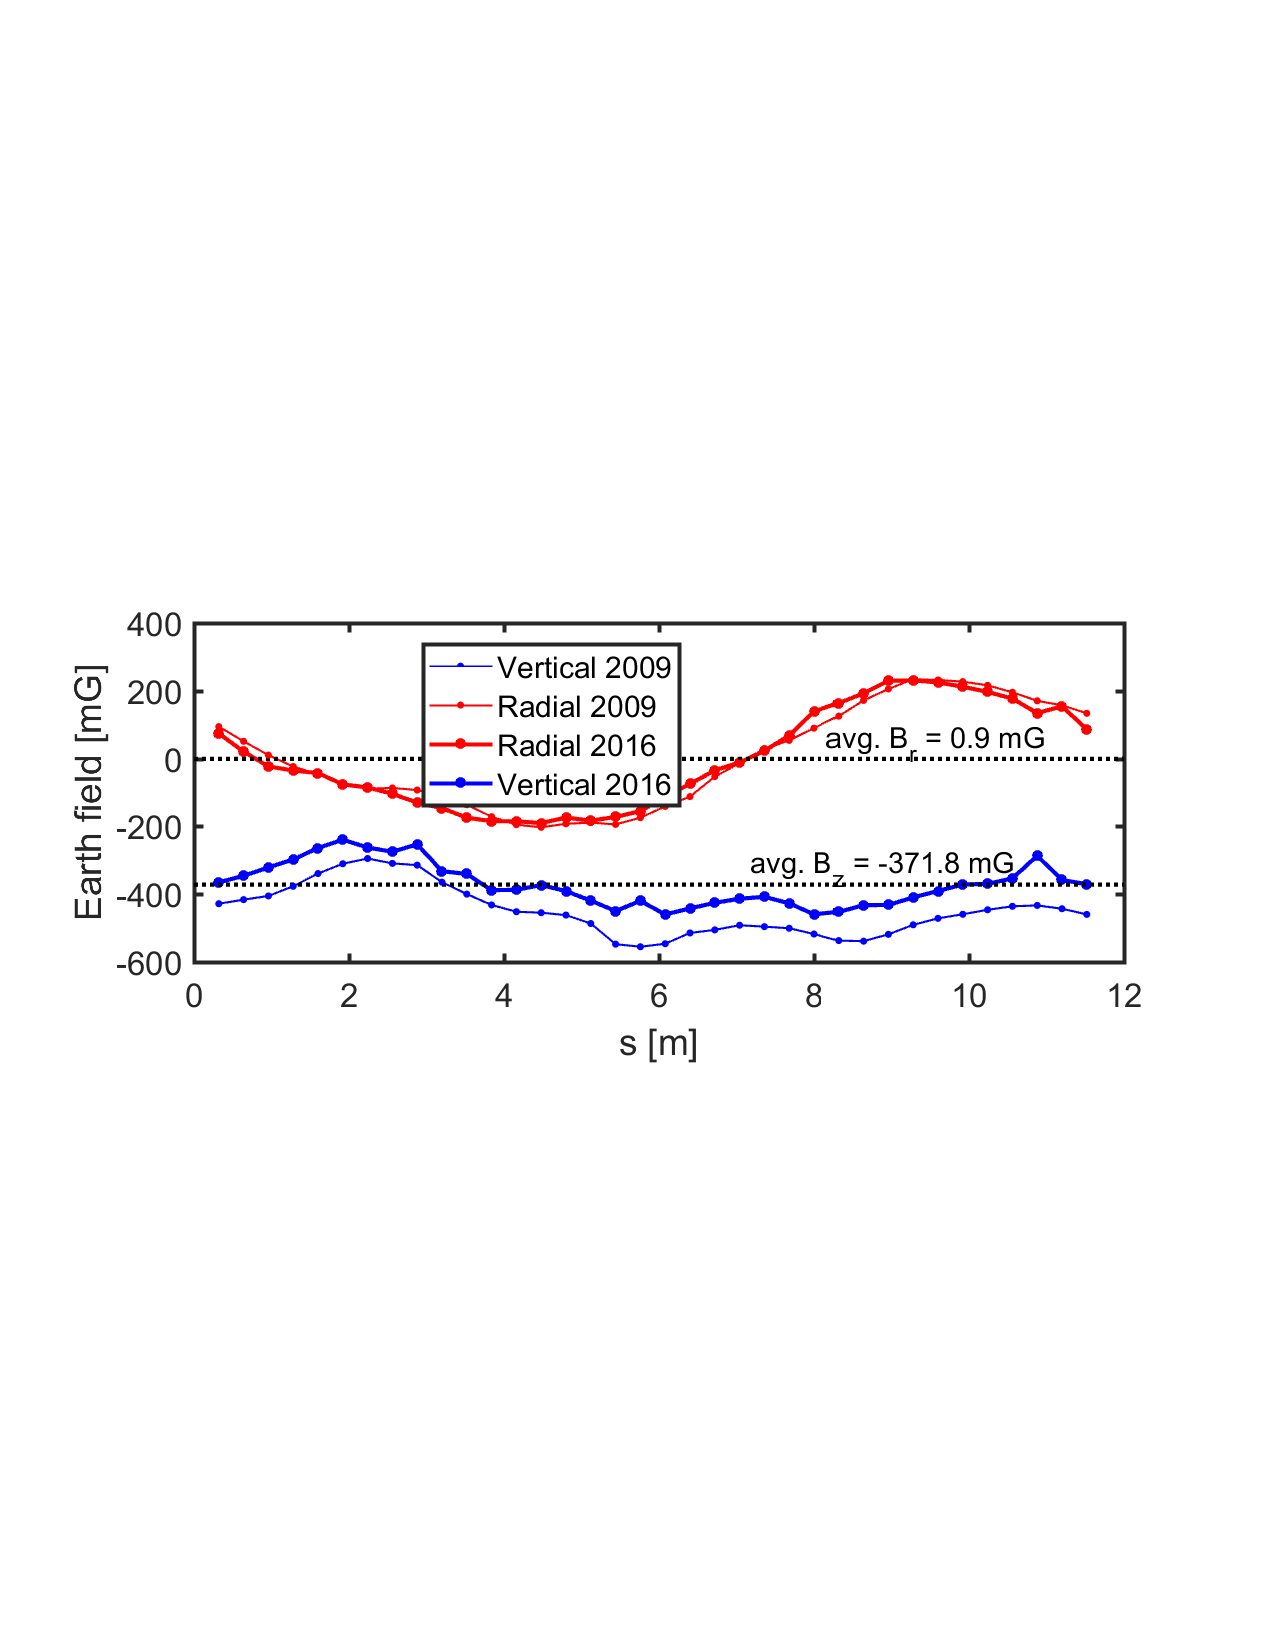
\includegraphics[width=\textwidth]{6.figures/earth_field_new.png}
\end{center}
\renewcommand{\baselinestretch}{1}
\small\normalsize
\begin{quote}
\caption[]{Ambient fields measured at UMER dipoles, from Dave Sutter measurements 6/1/2010 and 7/22/2016.}
\label{fig:earthfield}
\end{quote}
\end{figure} 
\renewcommand{\baselinestretch}{2}
\small\normalsize

\begin{figure}
\begin{center}
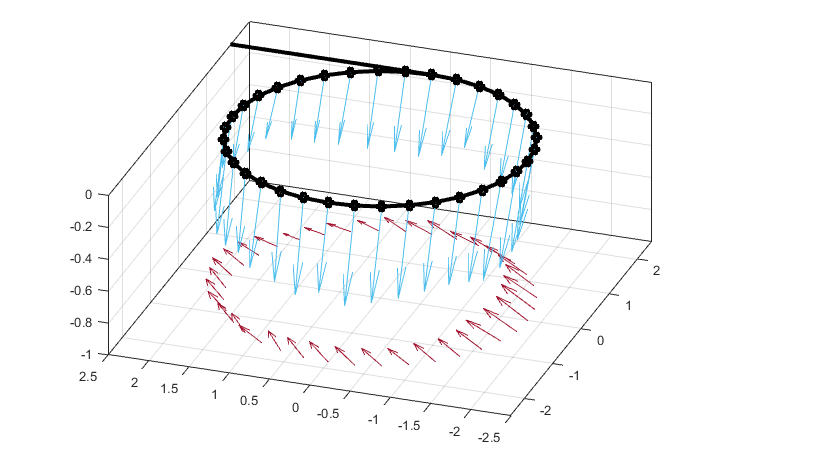
\includegraphics[width=\textwidth]{6.figures/earth_field_3D.png}
\end{center}
\renewcommand{\baselinestretch}{1}
\small\normalsize
\begin{quote}
\caption[]{Ambient field data vectors, including xy projection. x,y units are meters, z-axis is milli-Gauss.}
\label{fig:earthfield3D}
\end{quote}
\end{figure} 
\renewcommand{\baselinestretch}{2}
\small\normalsize


Because the beam is immersed in a bending field, in the perfectly aligned case a beam orbit that is centered in the quadrupoles is required to be displaced in the BPMs, as in Fig. \ref{fig:BPMcartoon}. Simple calculations with a constant background field show that we expect the ideal orbit to be radially displaced by [todo:]. However, in the case of azimuthally-varying ambient fields and displacements up to several millimeters, we expect larger displacements of the "best-possible" orbit.

\begin{figure}
\begin{center}
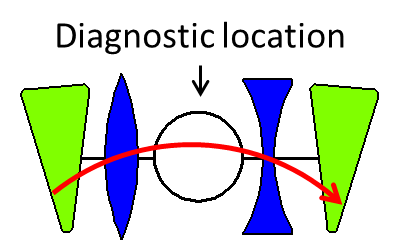
\includegraphics[width=0.5\textwidth]{6.figures/bpm_quads_cartoon.png}
\end{center}
\renewcommand{\baselinestretch}{1}
\small\normalsize
\begin{quote}
\caption[]{Diagram of beam position in diagnostic (BPM) for an orbit that is horizontally centered in the quadrupoles.}
\label{fig:BPMcartoon}
\end{quote}
\end{figure} 
\renewcommand{\baselinestretch}{2}
\small\normalsize

Steering in the ring is controlled by 36 horizontal bending dipoles, which determine the shape of the horizontal closed orbit, and which can be independently adjusted to optimizie the orbit. This is different from the typical case of a larger ring, which uses fixed dipoles and adjustable corrector magnets. There is 1 independent horizontal dipole every 2 quadrupoles.  Vertical correction is made with 18 printed circuit corrector magnets located at pipe flanges, which are named "RSV" magnets. There is 1 RSV corrector every 4 quadrupoles. Additional vertical correctors have been added and proposed, as described in Section \ref{sec:steering:vertical}. Steering near injection is controlled by 6 vertical and horizontal corrector magnets in the injection line, in the "SDH" and "SDV" families. Additionally, there are two correctors (one horizontal and one vertical) in the ring near the intersection of the injection pipe (the "Y-section"), named "SDR6H" and "SDR6V." 







\section{UMER Steering Magnets}

\begin{table}[h]
\centering
\caption{UMER Steering magnet strengths}
\label{tab:UMERsteererstrength}
\begin{tabular}{|c|c|c|c|c|}
\hline
Magnet Name & length [cm] & radius [cm] & Integ. Field / A [G-cm/A] & strength [$^o$/A] \\
BD & 4.44 & 2.87 & 19.917& 3.37 \\
PD & 4.40 & 4.40 & 1.913 & 0.32 \\
RSV& 3.80 & 5.75 & 3.886 & 0.66 \\
SD & 2.37 & 4.73 & 3.317 & 0.56 \\
SSV& 1.54 & 2.79 & 3.627 & 0.61 \\
\hline
\hline
\end{tabular}
\end{table}


\begin{figure}
\begin{center}
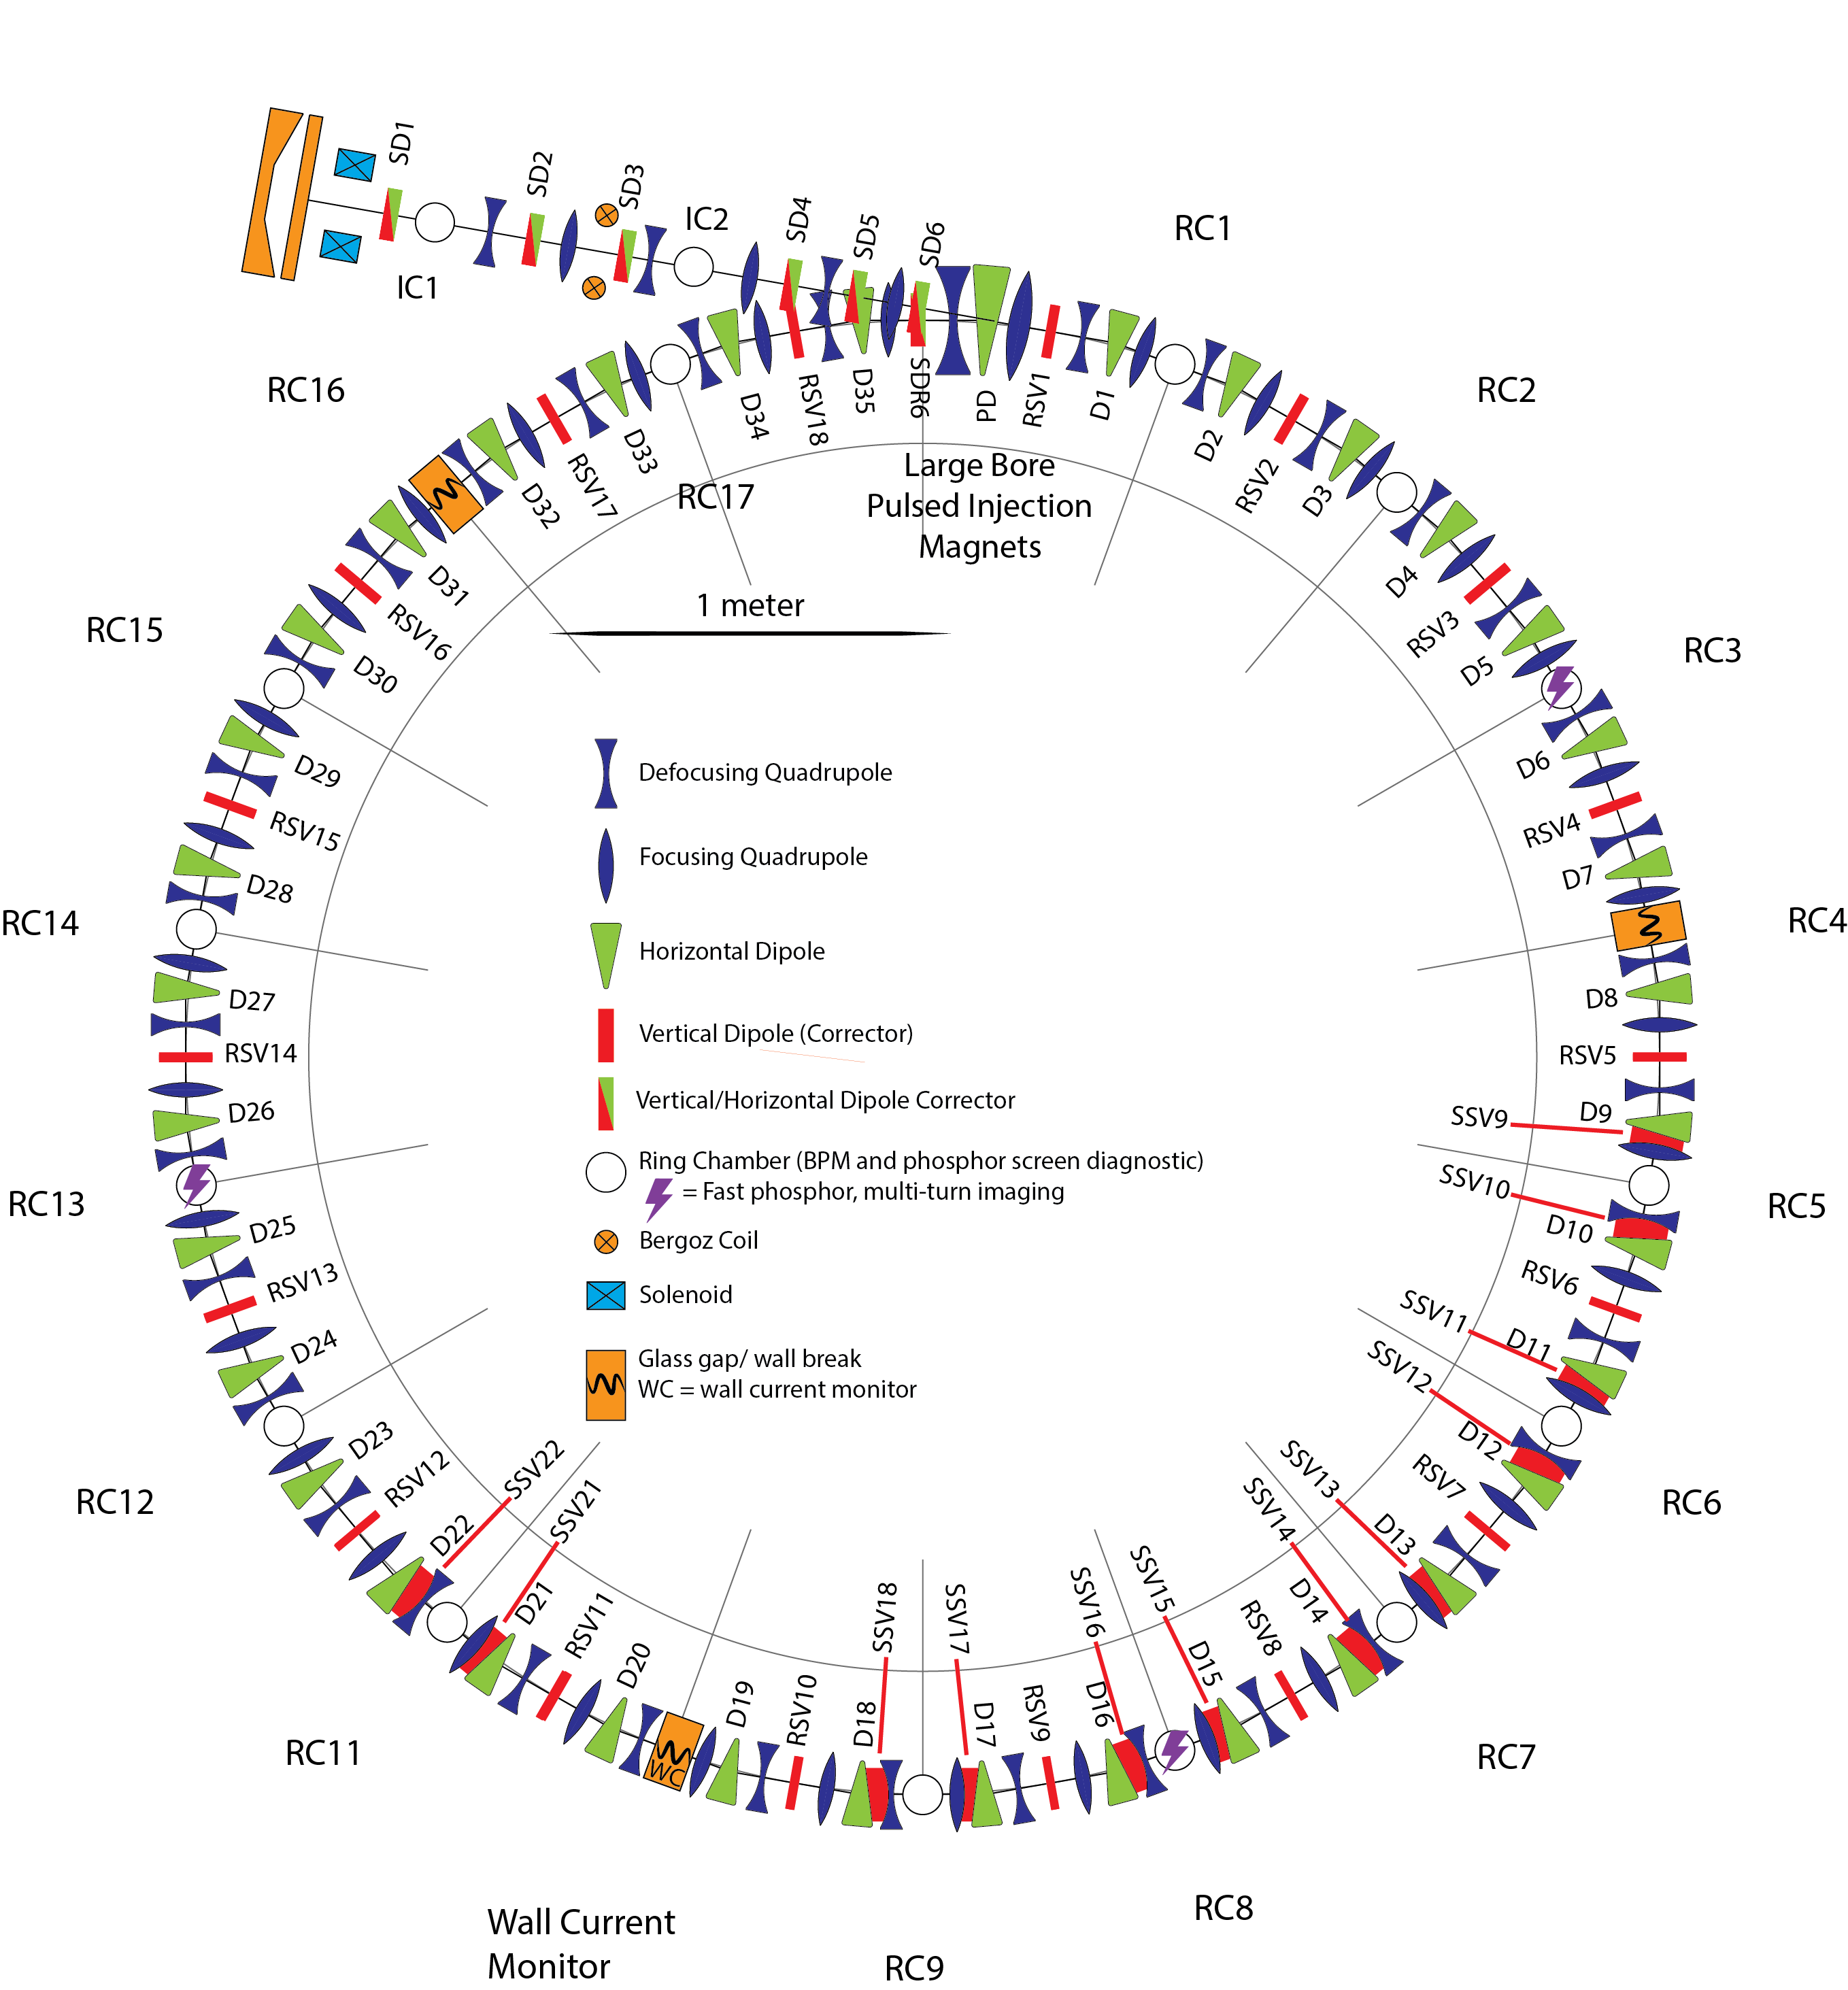
\includegraphics[width=\textwidth]{6.figures/full_ring_steerers_labelled.png}
\end{center}
\renewcommand{\baselinestretch}{1}
\small\normalsize
\begin{quote}
\caption[]{UMER Diagram with all steerers labelled. SSV family is discussed in Section \ref{sec:steering:SSV}}
\label{fig:steerers-labelled}
\end{quote}
\end{figure} 
\renewcommand{\baselinestretch}{2}
\small\normalsize



\section{Prior Approach}

%todo: recap Chao thesis?



% New Approach
An alternative approach to steering was developed using a steering procedure with local corrections to ensure the equilibrium orbit is centered (or as close to centered as possible) in the quadrupoles. This is unique from the response matrix method, in which a global correction is calculated that aims to center the equilibrium orbit at the 14 BPM locations. The steering algorithm is a methodical, "front to back" approach that first minimizes the position of the beam in the quadrupoles on the first turn then minimizes orbit deviations in subsequent turns. This algorithm should result in smaller local orbit excursions from quadrupole centers, since it utilizes 36 position data points at quadrupole locations for the first turn orbit as opposed to 14 at the BPMs.
This is proposed as a alternative to the response matrix steering algorithm \cite{KPRnote:2011}, and may be more useful for applications where orbit centering in the quadrupoles is essential.

The remainder of this chapter describes the tools and algorithmic approach to centering the first turn orbit in the quadrupole centers. First I describe the quad-as-BPM procedure for measuring first-turn centroid position at the quadrupoles (Section \ref{sec:steering:quad-as-bpm}). Then I summarize the application of various algorithms to set horizontal and vertical steerers in Section \ref{sec:steering:ringsteering}, including theoretical "best-case" orbit excursions and proposed vertical steering upgrades to meet the dynamic aperture requirements for the nonlinear optics experiments. This includes first-turn data taken during ring steering tests.
Section \ref{sec:steering:implementation} lays out a sample steering procedure, including injection and multi-turn optimization routines. 



 

 



\section{Steering Algorithms} \label{sec:steering:steeringalgorithm}




\subsection{Horizontal Steering Algorithm}

Horizontal orbit in the ring is controlled by 35 ring dipoles and the pulsed injection magnet (PD), for a ratio of 1 corrector per 2 quads. As the ring dipoles are designed to bend the beam $10^o$, they are sufficient to correct the background Earth field, which on average bends the beam $\approx 2.1^o$ per cell. 

I applied VRUMER simulation to determine an effective algorithm for minimizing first turn orbit position in the quadrupoles by setting the 36 dipoles. As there are 2 quadrupoles per dipole, there are a variety of minimization functions available (aim for the center of either quadrupole, or some weighted combination of the two). I only considered quadrupoles immediately downstream of a given dipole, upstream of the next dipole. In these cases, multiple passes would be necessary to find a "centered" orbit, and relaxation is slow. The 2 downstream quadrupoles are indicated as focusing "F" or defocusing "D" based on polarity in the horizontal plane. The nearest downstream quadrupole for any dipole is focusing (in the standard FODO configuration), an sketched in Fig. \ref{fig:BPMcartoon}.
 
I considered steering algorithms with an angle term $x'$. In the thin lens approximation for a focusing dipole separated from a defocusing dipole by a drift of distance $L$, $x'_F \equiv \frac{x_D-x_F}{L}$. I used $x'_F \propto x_D-x_F$ to include $x'_F$ in the RMS minimization term, see Table \ref{tab:algorithm}.

\begin{table}[h]
\centering
\caption{Different algorithms and their performance (RMS position in quads) for initial condition $x=1$mm, $x'=0$. }
\label{tab:steeringalgorithm}
\begin{tabular}{|l|l|c|c|c|}
\hline
shorthand & Minimization function & RMS($x_Q$) [mm] & RMS($x_Q$) [mm]  & plot trace \\
& & no misalign. & $\sigma=5$mm & \\
\hline
$x_F$ & $\| x_F \|$ & 5.3 & 37.3 & {\color{blue} $\circ$} \\
$x_D$ & $\| x_D \|$ & 0.2 & 6.9 & {\color{red} $\triangle$} \\
$x_F,\thinspace x_D$ & $\sqrt{x_F^2+x_D^2}$ &  2.1 & 9.3 & {\color{cyan} $\diamond$} \\
$x_F,\thinspace x'_F$ & $\sqrt{x_F^2+(x_D-x_F)^2}$ & 0.2 & 6.6 & $\ast$ \\
$x_D,\thinspace x'_F$ & $\sqrt{x_D^2+(x_D-x_F)^2}$  & 0.2 & 7.0 & {\color{magenta} $+$} \\
\hline
\end{tabular}
\end{table}




\begin{figure}[!htb]
\centering
\subfloat[No misalignments]{
	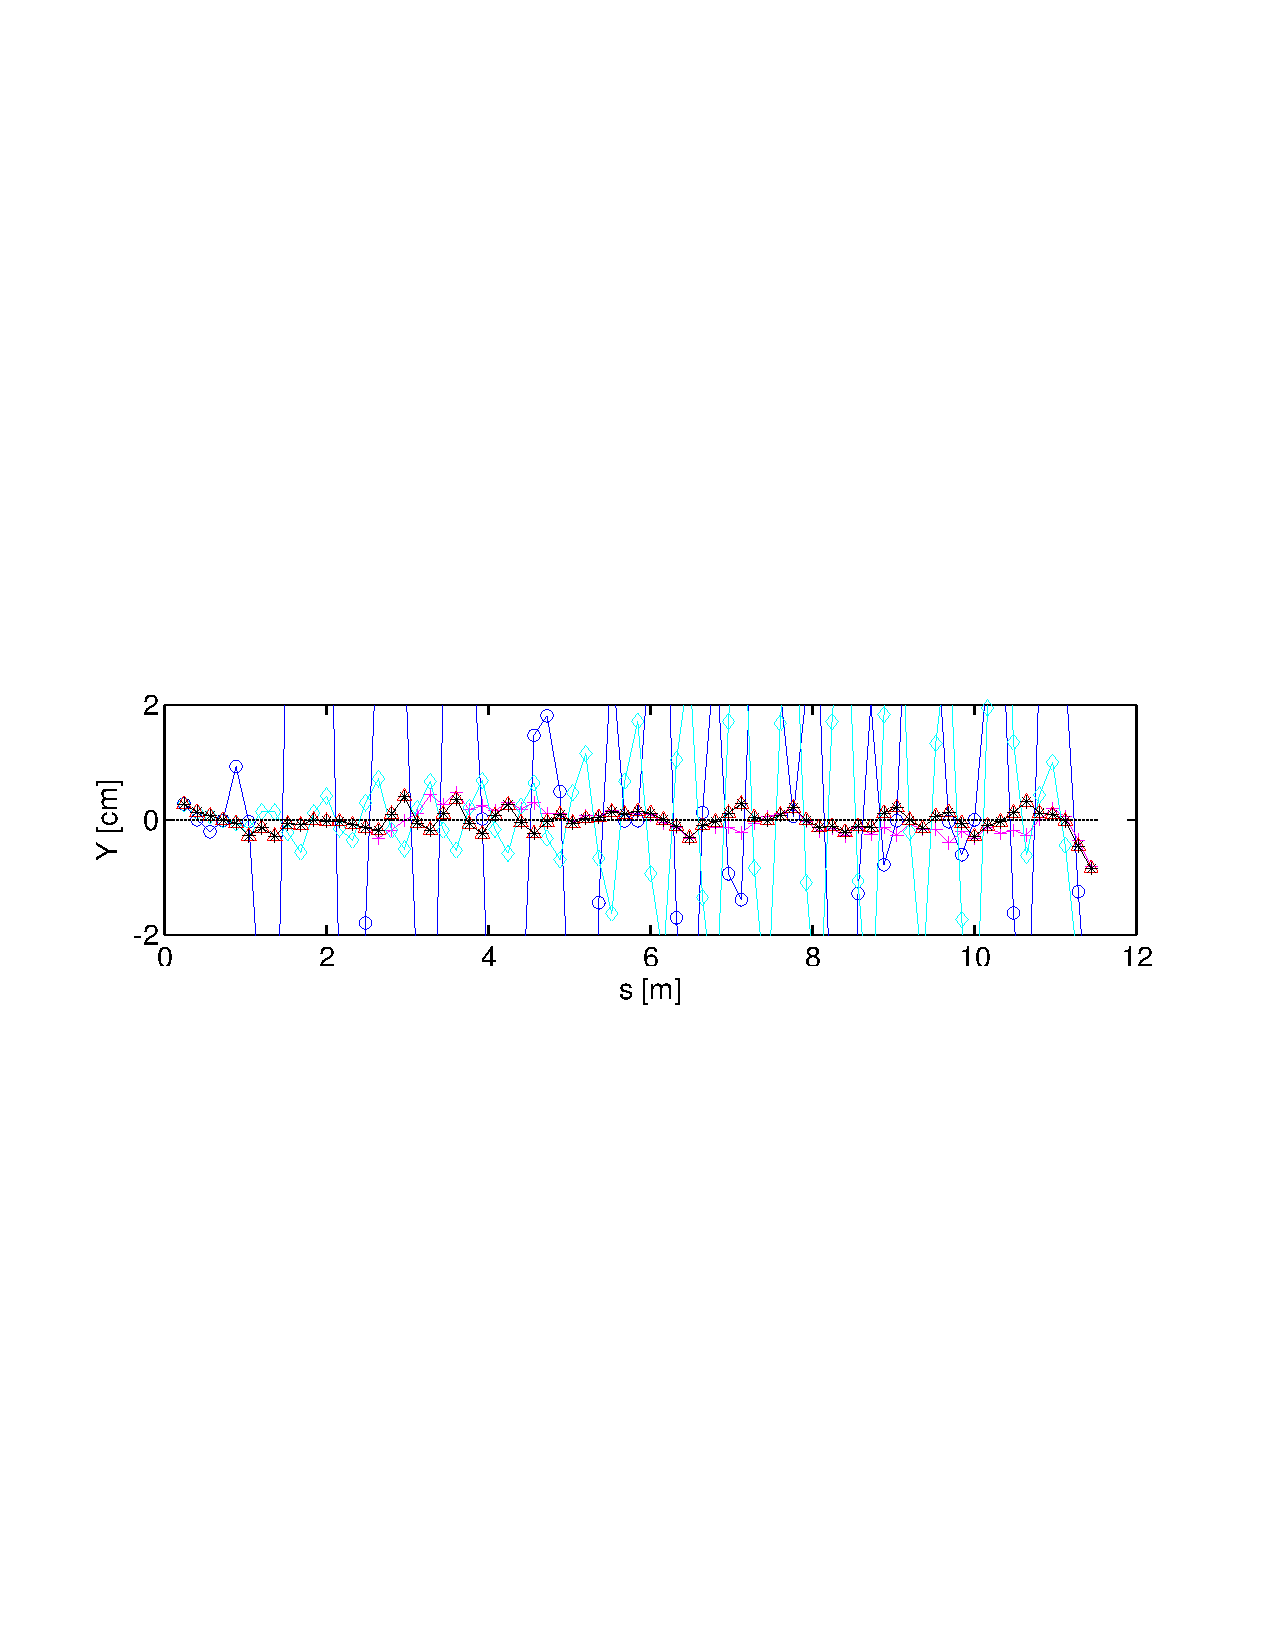
\includegraphics[width=\textwidth,trim={.5in 4.3in .7in 4.5in},clip]{6.figures/vrumer_steering_algorithm_compare_x1_xp0.pdf}}
\hspace{.05in}
\subfloat[Random quad misalignments from Gaussian distribution, $\sigma=5$mm]{
	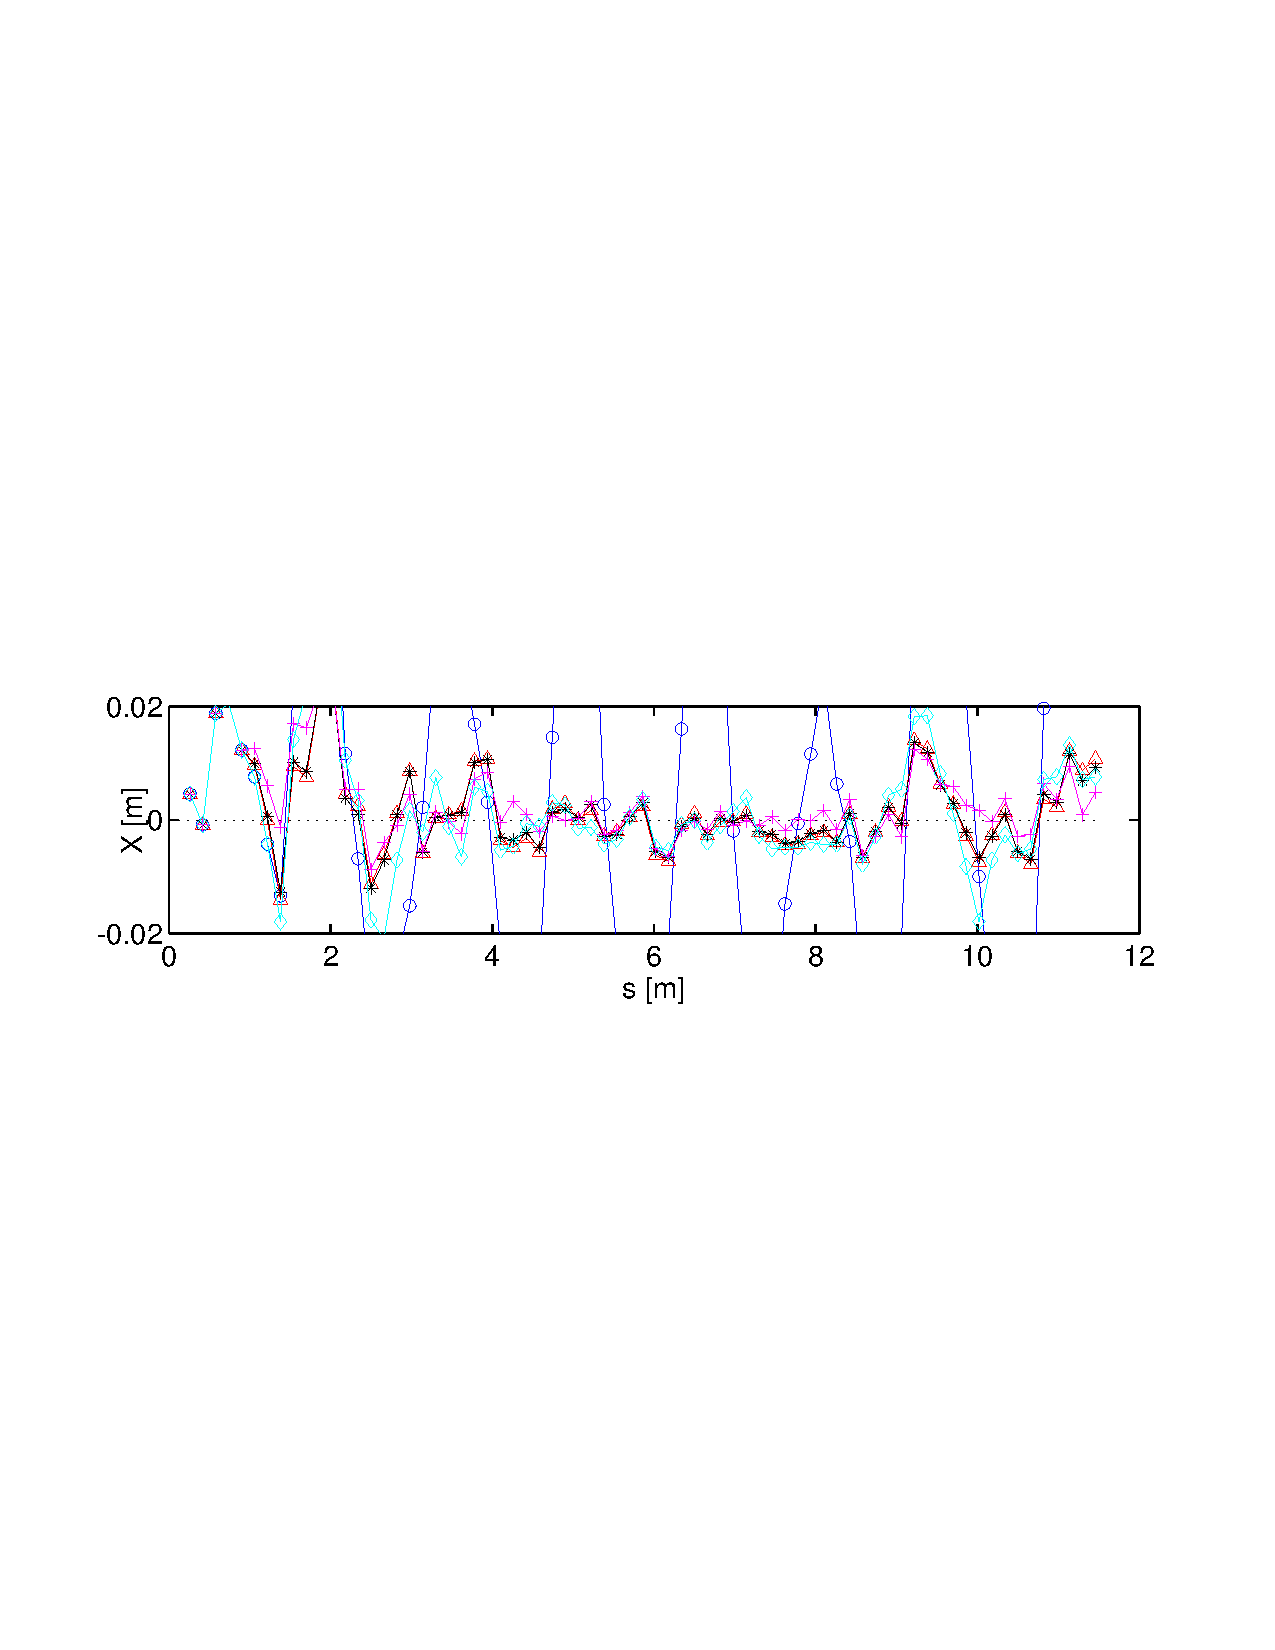
\includegraphics[width=\textwidth,trim={.5in 4.3in .7in 4.5in},clip]{6.figures/vrumer_steering_algorithm_compare_x1_xp0_sig5.pdf}}
\caption{First turn VRUMER orbits for initial condition $x=1$mm, $x'=0$. 
%blue circle: $x_F$, red triangle: $x_D$, black asterisk: $x_F$,$x'_F$, 
%magenta plus:  $x_F$,$x'_F$, green diamond: $x_F$,$x_D$
}
\label{fig:steeringalgorithm}
\end{figure}




The results of multiple steering algorithms are shown in Table \ref{tab:steeringalgorithm}. Simulated orbits with and without misalignment errors are shown in Fig. \ref{fig:steeringalgorithm}. Qualitatively, the best performers were $x_D$, $x_F$,$x'_F$, $x_D$,$x'_F$, resulting in almost identical orbits (sub-millimeter differences) that converge very quickly towards the center of the quads given an injection error or quad misalignment.

In the lab, it is much faster to minimize $x_D$, as the data collection is faster. It also allows interpolation between scanned dipole settings, as the data can be fit to a line and the zero-crossing calculated (the RMS minimization functions do not lend themselves to fitting by a simple function). 
However, when applied in the lab, the $x_F$,$x'_F$ algorithm seems to yield better results. 
This may be because of its ability to handle relative misalignments between the focusing and defocusing quadrupoles, as well as reduced sensitivity to nonlinearities in the quad fields and BPM response for large centroid positions. 
For implementation in the lab (described in Section \ref{sec:steering:implementation}), I chose to use $x_D$ as the minimization function, due to faster steering time.





\subsection{Vertical Steering Algorithm}

Vertical steering in UMER is accomplished by 18 vertical correction magnets (RSV's) located at the pipe flanges every $20^o$. All of these magnets are fairly weak (see Table \ref{tab:UMERsteererstrength}) and spaced half as densely as horizontal correctors.  The largest source of vertical alignment errors is the radial component of the Earth's field, shown in Fig. \ref{fig:earthfield}. Although the amplitude 200 mG is comparable to the vertical field, the average is only $<1$ mG.

I use VRUMER to test various vertical steering algorithms and place a lower bound on the best possible first turn orbit using existing vertical steerers, results are shown in Table \ref{tab:vert_algorithm}. I considered three test cases:

\begin{itemize} 
\item Ideal: Perfect alignment, RSV current constrained to be $\le10$ A. 
\item SV limit: Perfect alignment, RSV current limited to $\le2$ A.
\item Misaligned: Random misalignment, from Gaussian distribution $\sigma=1$ mm, RSV current limited to $\le2$ A.
\end{itemize}


\begin{table}[!htb]
\centering
\caption{Vertical steering algorithms and their performance (RMS position in quads) for perfect alignment. Subscript indicates quad \# counting downstream from vertical steerer ($y_1$ is position in first quad downstream from each RSV).}
\label{tab:vert_algorithm}
\begin{tabular}{|l|l|c|c|c|}
\hline
shorthand & Minimization Function & RMS($y_Q$) [mm] & RMS($y_Q$) [mm] & RMS($y_Q$) [mm] \\
& & & SV limit & $\sigma = 1$mm \\
\hline
SV=0 & none  & 4.6 & 4.6 & 10.4 \\ \hline
$y_1$& $\| y_1 \|$ & 37.0 & & \\
%$y_2$& $\| y_2 \|$ & & & \\
$y_3$& $\| y_3 \|$ & 1.5& 2.2 & 3.8\\
$y_4$& $\| y_4 \|$ &  1.7& 2.5 & 3.4\\ \hline
$y_1$,$y_2$ & $\sqrt{\frac{1}{2}\left(y_1^2 +y_2^2\right)}$ &  25.9 & & \\
$y_2$,$y_3$ & $\sqrt{\frac{1}{2}\left(y_1^2 +y_3^2\right)}$ &  1.2& 2.5 & 4.2\\
$y_3$,$y_4$ & $\sqrt{\frac{1}{2}\left(y_3^2 +y_4^2\right)}$ &  0.98 & 2.4 & 3.7 \\
$y_1$,$y_3$ & $\sqrt{\frac{1}{2}\left(y_1^2 +y_3^2\right)}$ &  1.1 & 2.5& \\
(focusing) & & & & \\
$y_2$,$y_4$ & $\sqrt{\frac{1}{2}\left(y_2^2 +y_4^2\right)}$ &  0.93 & 2.6& 4.6\\
(defocusing) & & & & \\ \hline 
$y_1$,$y'_1$ & $\sqrt{\frac{1}{2}\left(y_1^2 +(y_2-y_1)^2\right)}$ & 18.7 & & \\
$y_2$,$y'_2$ & $\sqrt{\frac{1}{2}\left(y_2^2 +(y_3-y_2)^2\right)}$ & 1.1 & 2.2& \\
$y_3$,$y'_3$ & $\sqrt{\frac{1}{2}\left(y_2^2 +(y_4-y_3)^2\right)}$ & 1.3 & 2.2& \\
$y_1$,$y_2$,$y_3$,$y_4$ &  $\sqrt{\frac{1}{4}\left(y_1^2 +y_2^2+ y_3^2 +y_4^2\right)}$ & 0.95 & 2.4 & 5.0\\
\hline
\end{tabular}
\end{table}

In summary, in the ideal case (strong correctors, no mechanical misalignments), we can obtain vertical steering with $\max{(y)} \sim 3$ mm, rms$(y) \sim 1$ mm (Fig. \ref{fig:SV_y4}). This requires maximum RSV currents in the range 3-4 A, which is not possible given exiting heat dissipation limits.  If we restrict ourselves to 2 A in the RSVs, the best possible solution is $\max{(y)} \sim 7$ mm, rms$(y) \sim 2$ mm (Fig. \ref{fig:SV_y4_CL}). Additionally, allowing for random vertical misalignments of order 1 mm, this increases to $\max{(y)} \sim 10$ mm, rms$(y) \sim 3-4$ mm (Fig. \ref{fig:SV_y4_misalign}).

I conclude that the existing vertical correcters provide too weak of a correction to offer significant improvement on the existing first-turn solution. Enhanced vertical correction is necessary to achieve steering comparable to horizontal plane. This is possible through the use of radial field-cancelling Helmholtz coils or through addition of more weak vertical correctors (see Section \ref{sec:steering:SSV}). 


\begin{figure}[!htb]
\centering
\subfloat[Vertical steering for perfect alignment, no current limit. Steering by minimizing $\| y_4 \|$. Red dotted trace is vertical solution without steering corrections.]{
     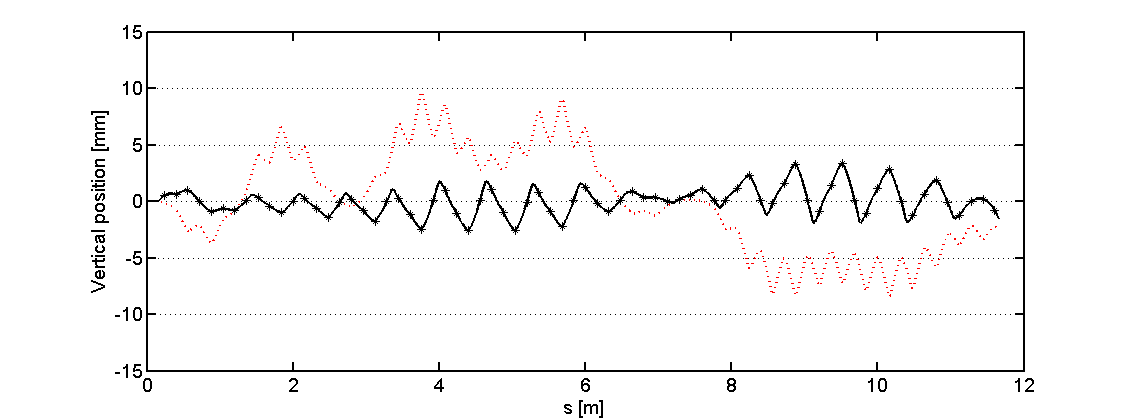
\includegraphics[width=.8\textwidth]{6.figures/steering_rms_y4.png}
     \label{fig:SV_y4}}
\hspace{0.5in}
\subfloat[Vertical steering for perfect alignment, RSV current limited to 2 A. ]{
     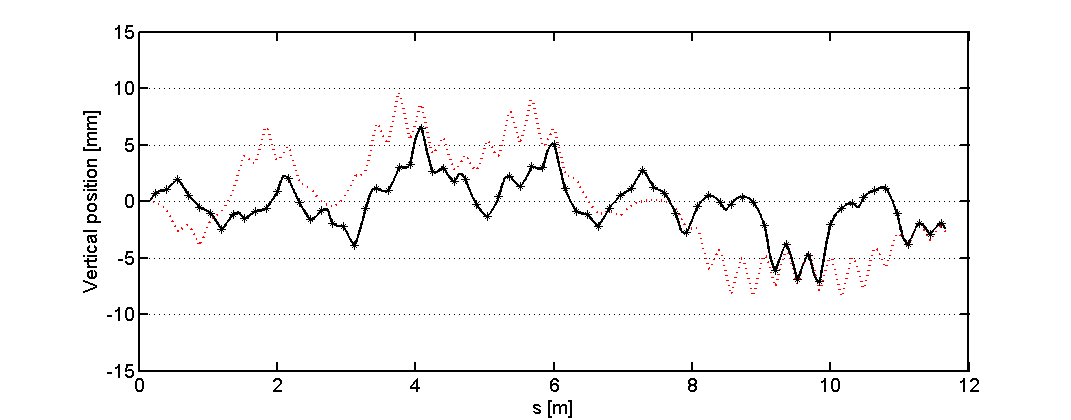
\includegraphics[width=.8\textwidth]{6.figures/steering_rms_y4_CL.png}
     \label{fig:SV_y4_CL}}
\hspace{0.5in}
\subfloat[Vertical steering for misalignment of $\sigma=1$ mm, RSV current limited to 2 A.]{
     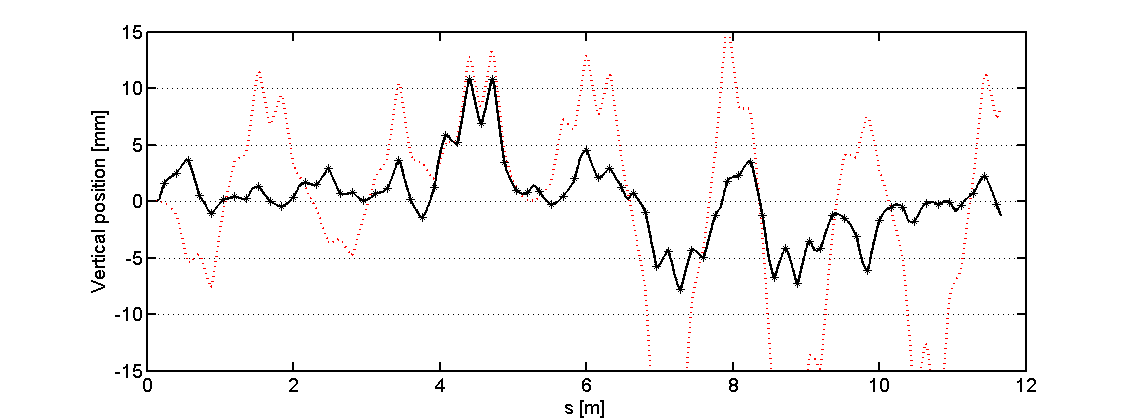
\includegraphics[width=.8\textwidth]{6.figures/steering_rms_y4_misalign1.png}
     \label{fig:SV_y4_misalign}}
\end{figure}



\begin{table}[h]
\centering
\caption{Statistics for quad-centering steering method.}
\label{tab:steeringresults}
\begin{tabular}{|l|c|c|}
& Horz. & Vert. \\
\hline
First turn RMS & & 1.32 mm\\
First turn Max & & 4.05 mm\\
Four turn RMS (in BPMs)& & \\
Four turn Max (in BPMs)& & \\
\hline
\end{tabular}
\end{table}








 





\subsubsection{Corrected Beam Orbit}


%todo: newer data would be nice
\begin{figure}[h]
\centering
\subfloat[Vertical position of 6 mA beam in quads for 1st turn.]{\label{fig:vertical_quads}
	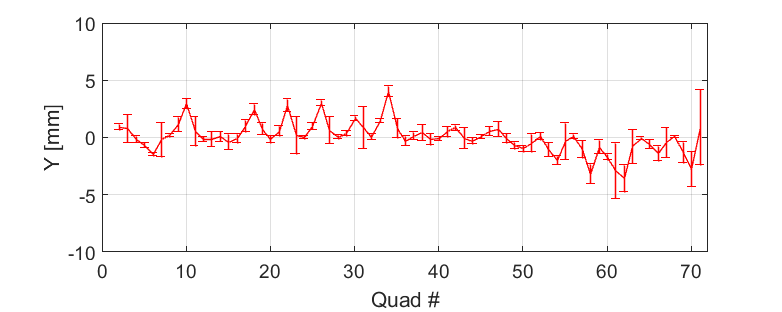
\includegraphics[width=\textwidth]{6.figures/steering-y-170901.png}}
\hspace{.05in}
\subfloat[OLD REPLACE PLS, Vertical position of 6 mA beam in BPMs for first 4 turns. Note shorted vertical plates at RC2, RC11.]{\label{fig:vertical_BPMs}
	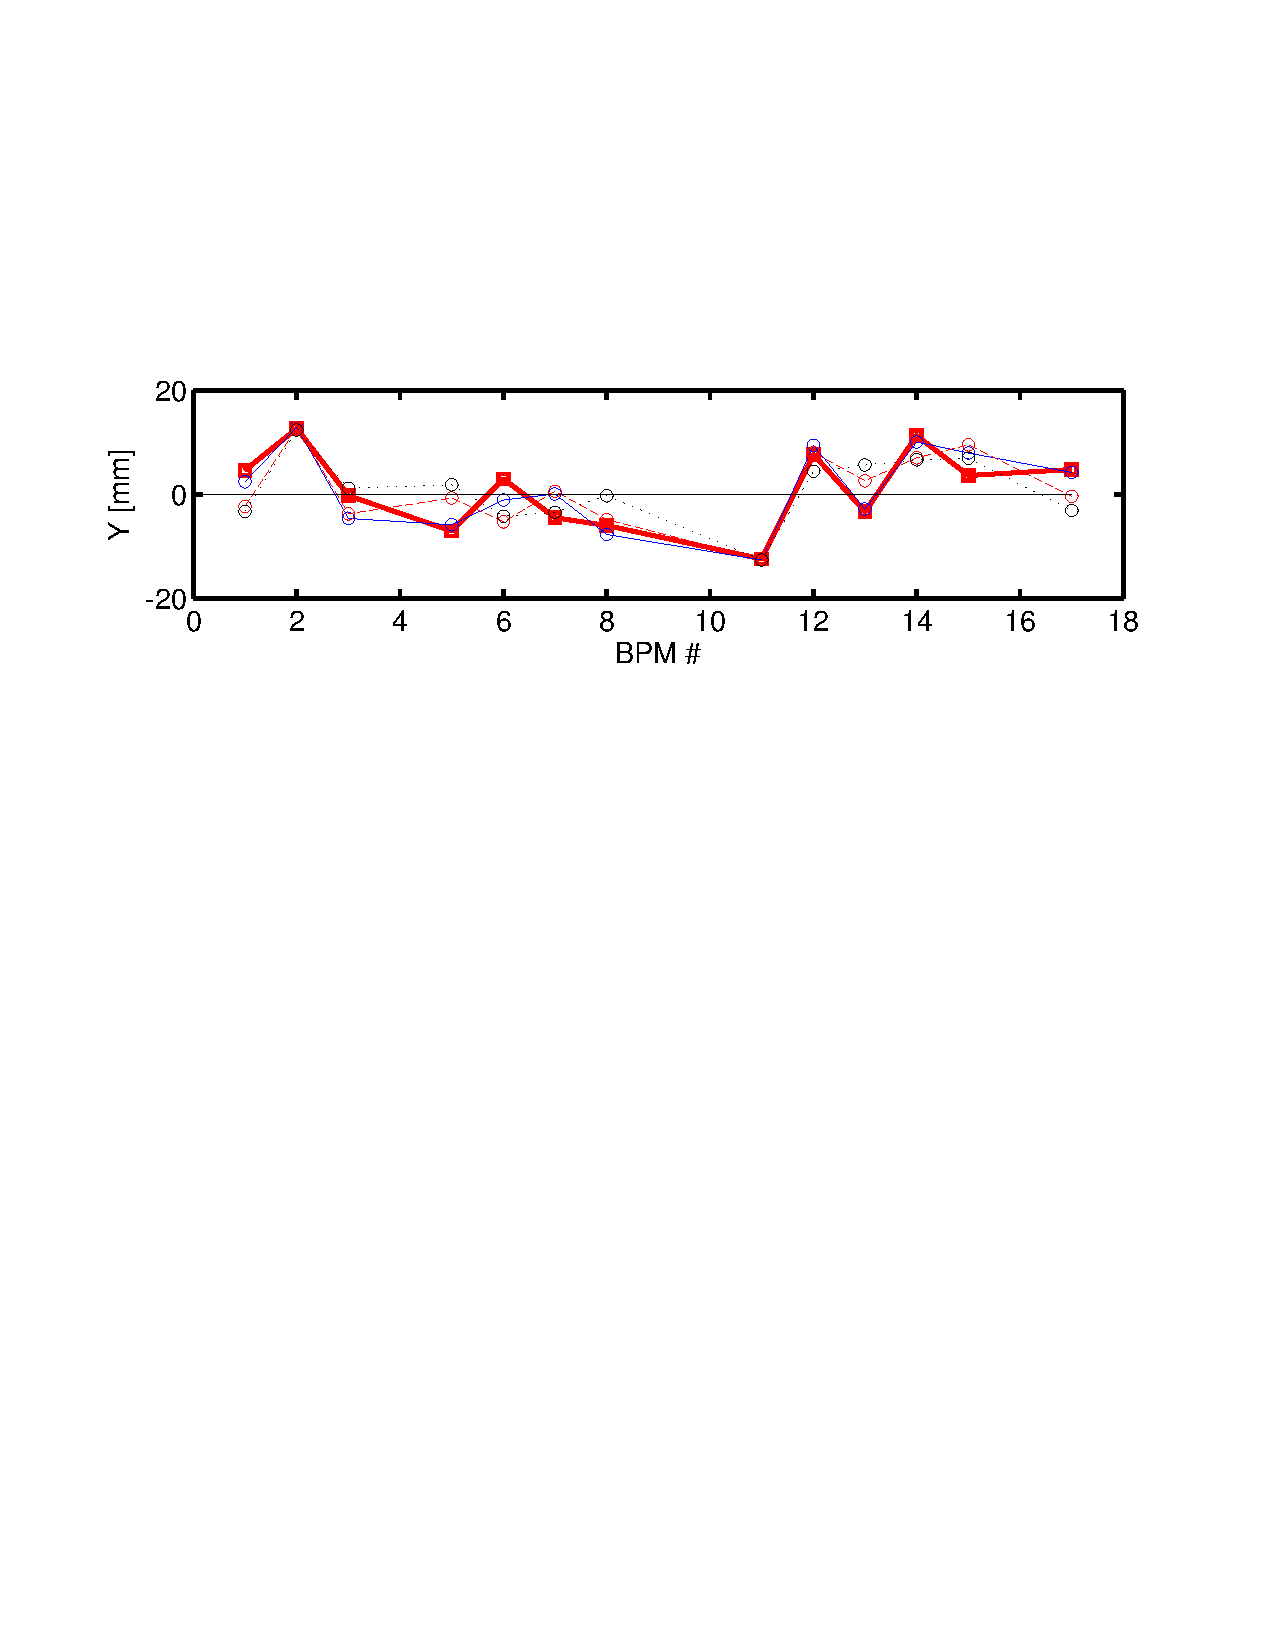
\includegraphics[width=\textwidth,trim={.5in 6.5in .5in 2.4in}, clip]{6.figures/BPM_position_sol151116_Y.pdf}}
\end{figure}


\section{Increasing Vertical Steering Capability} \label{sec:steering:SSV}

Vertical orbit correction is inherently limited by the strength of vertical corrector magnets, RSV in Table \ref{tab:UMERsteererstrength}.
Previous assumption has been that sparsely populated, low-field vertical correctors were sufficient to correct for the low average radial field. However, at regions of locally high radial field, the radial field bends $\approx 2.1^o$ per vertical corrector (every 2 ring cells), while the corrector at maximum safe excitation of 2 A can only supply $1.2^o$ of correction. This results in locally high vertical excursions, as seen in Fig. \ref{fig:vertical_quads} and Fig. \ref{fig:vertical_BPMs}. In the first turn, the maximum vertical displacement from quad center is 10 mm and the RMS displacement is 3.2 mm. 
%Deviation about this orbit in the first 4 turns is $\sim10$ mm. 

% This is much worse than the best horizontal steering solution described in this note. For horizontal beam position, the first-turn orbit (Fig. \ref{fig:ring_steering}) exhibited maximum horizontal displacement of 3.1 mm and RMS displacement of 0.8 mm. Deviation about this orbit in the first 4 turns is $\sim2$ mm. 

While good recirculation with small turn-to-turn oscillation amplitude is possible using the existing correctors, alignment of the orbit to the vertical center of the quads is limited by the strength and density of vertical correctors. In other words, the beam can be injected with minimum deviation from the closed orbit, but this orbit has large deviations ($\ge 5$ mm) from the quadrupole centers.  


\begin{figure}[]
\centering
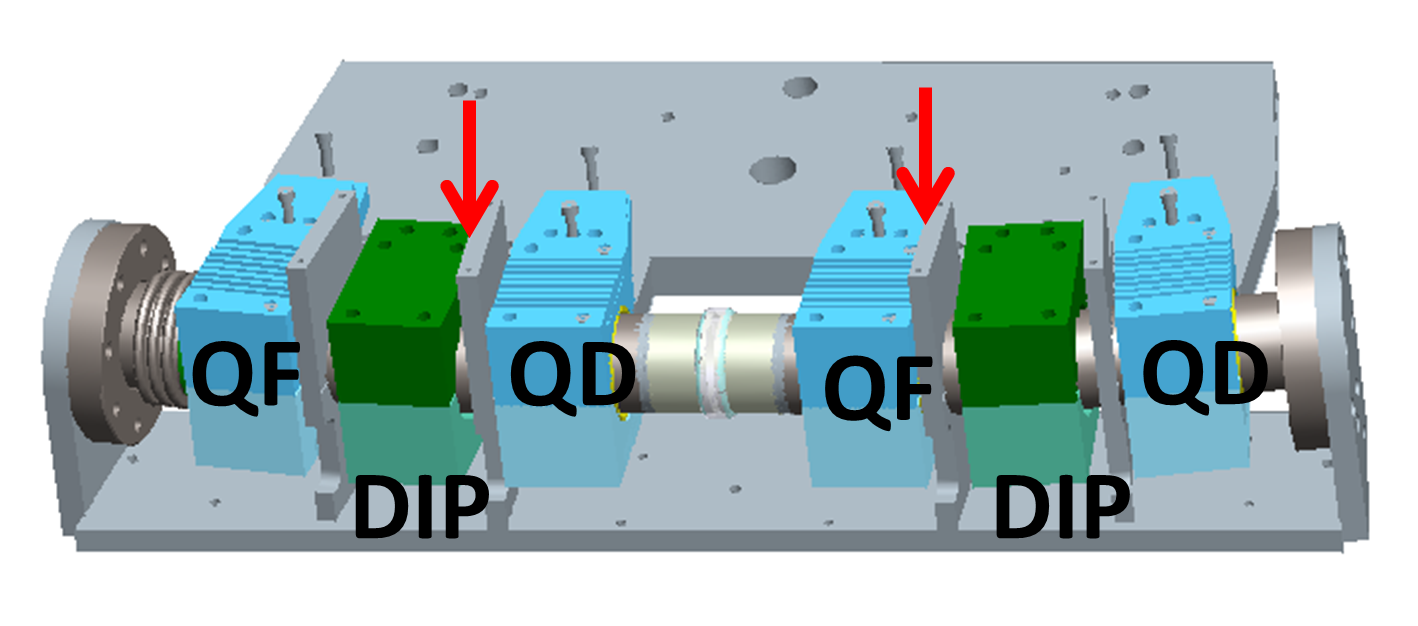
\includegraphics[width=0.5\textwidth]{6.figures/SSV/SSVlocations.png}
\caption{Locations of SSV's on UMER $20^o$ plate indicated with arrows. RSV's are located at vacuum flanges at ends of $20^o$ section.}
\label{fig:SSVlocation}
\end{figure}

Increased strength and/or density is required for vertical orbit control comparable to horizontal control. I tested the use of "Short Steerers," abbreviated SSV. These are short circuits of length [] that are used for orbit correction in the injection line, pictured in Fig. \ref{fig:SSVdrawing}. There is space in the dense UMER lattice for two additional SSV's per $20^o$ plate, as shown in Fig. \ref{fig:SSVlocation}. From Table \ref{tab:UMERsteererstrength}, the available correction of the SSV is $\approx 1.2^o$ per amp, comparable to RSV strength. With twice the density of the RSV, orbit correction should be sufficient for the $\approx 2.1^o$ of distortion per cell.

\begin{figure}[]
\centering
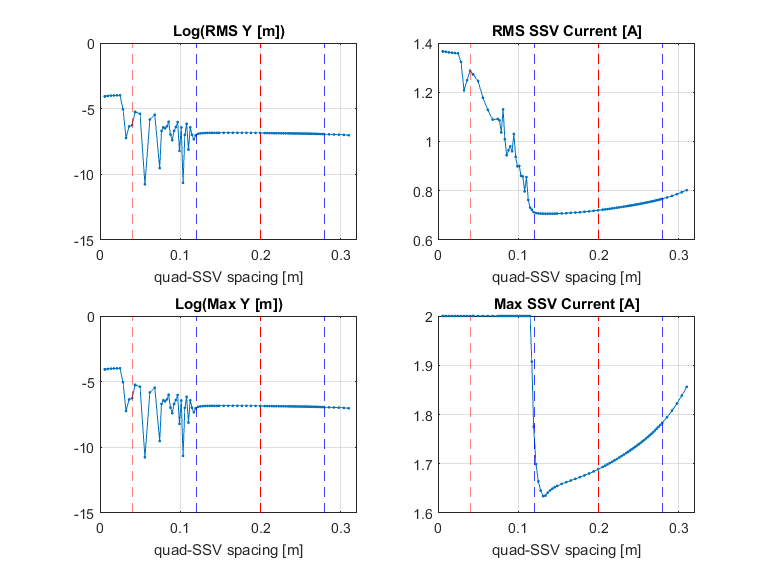
\includegraphics[width=0.75\textwidth]{6.figures/SSV/steering_behaviour_vs_lever_arm_distance.png}
\caption{Steering statistics for varying steerer-target distance. Quad center locations are indicated by dashed lines. Red dashes indicate distance from 1st SSV on $20^o$ plate, blue from 2nd SSV on $20^o$ plate.}
\label{fig:lever_arm}
\end{figure}

% \begin{wrapfigure}{r}{0.4\textwidth} 
% 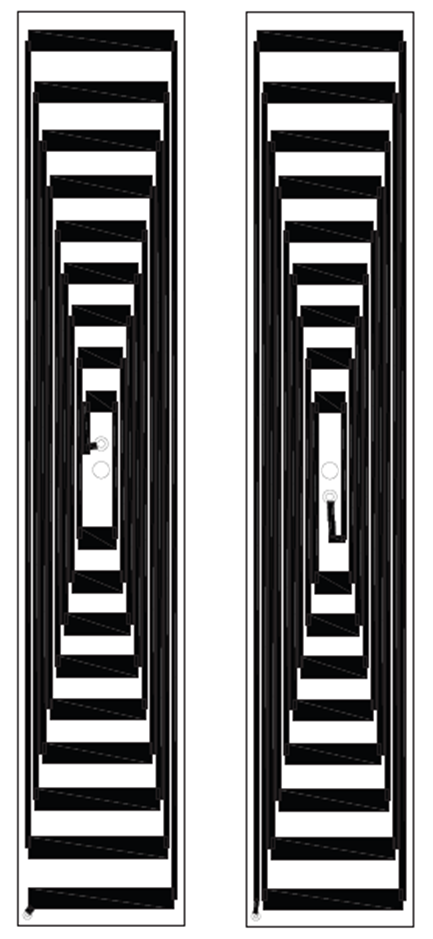
\includegraphics[width=0.4\textwidth]{6.figures/SSV/SSVdrawing.png}
% \caption{Circuit winding for SSV magnets.}
% \label{fig:SSVdrawing}
% \end{wrapfigure}


The target for steering with the SSV's is second downstream quadrupole, at a distance of $\approx 12$ cm from the SSV center. Dependence of SSV strength and correction on SSV-target separation is plotted in Fig. \ref{fig:lever_arm}. Similar to dipole steering, choice of "too-close" target leads to over-correction, reflected in the maximum SSV set-point which is at maximum safe current. Longer distances between steerer and target are necessary for corrections within the available strength, and there is a sharp transition between "good steering" and "poor steering" at $\approx 12$ cm. The target quadrupoles for the two SSV locations are at 20 cm and 28 cm respectively, within the range of good correction.


\begin{figure}[htb]
\centering
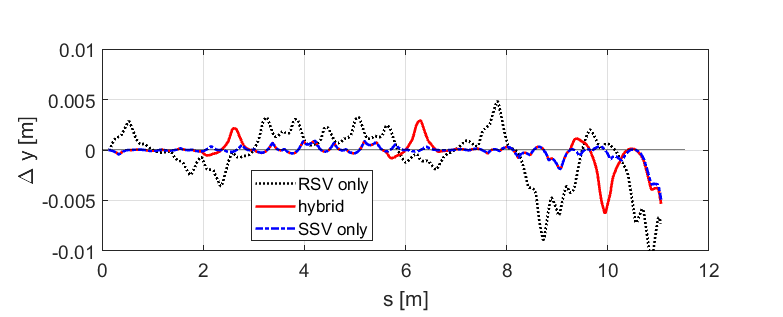
\includegraphics[width=0.75\textwidth]{6.figures/SSV/orbit_uneven_ssvs.png}
\caption{"Best-case" simulated orbits for quad-centered steering with just RSVs, hybrid (SSV's in 28 available locations, plot four RSV's for "glass gap" sections), and 36 SSV's}
\label{fig:SSVsimorbit}
\end{figure}

The resulting first turn orbit with SSV correction from VRUMER calculations is plotted in Fig. \ref{fig:SSVsimorbit}. There are three orbits plotted: orbit correction using only 18 RSV's (black dot), orbit correction using only 36 RSV's (blue dash), and orbit correction using 8 RSV's and 28 SSV's. In the ring, there are 4 $20^o$ sections with welded glass gap breaks in the pipe. Extra supports needed to protect the glass inhabit the available SSV space. In these sections, the two RSV's bookending the $20^o$ plate are also utilized. As seen in \ref{fig:SSVsimorbit}, there are large local deviations at the four glass gap sections.


\begin{figure}[htb]
\centering
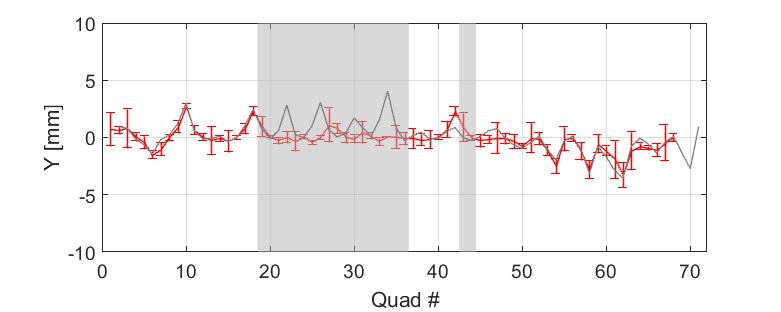
\includegraphics[width=0.75\textwidth]{6.figures/SSV/vert_steering_with_ssv_170831.png}
\caption{Measured first turn orbit for vertical steering with SSV's on 30\% of the ring (locations indicated by gray shading)}
\label{fig:SSVexporbit}
\end{figure}

The SSV's were very successful in simulation. To test their effectiveness in the lab, a trial run of 11 SSV's were installed on ring sections 5 - 11 (skipping section 10 due to glass gap in wall current monitor diagnostic). The SSV numbering system corresponds with the nearest horizontal dipole (SSV9 is immediately downstream of dipole D9, SSV10 upstream of D10, etc). The resulting first turn orbit, using the quad-centering algorithm with RSV1-5, SSV9-18, SSV21-22, RSV10-18 is plotted in Fig. \ref{fig:SSVexporbit}. Orbit statistics are in Table \ref{tab:SSVexporbit}. The addition of SSV's reduces the vertical orbit deviation by a factor of $\approx 2$, almost to a tolerance of $\pm 1$ mm.   

\begin{table}[h]
\centering
\caption{First turn orbit statistics for SSV trial run. Compare to vertical orbit in \ref{tab:steeringresults}}
\label{tab:SSVexporbit}
\begin{tabular}{|l|c|}
\hline
First turn RMS & 0.98 mm\\
First turn Max. & 3.25 mm\\
Shaded RMS & 0.45 mm\\
Shaded Max. & 1.11 mm \\
\hline
\end{tabular}
\end{table}



\section{Steering for alternative FODO lattice}


\section{Steering for single-channel octupole lattice}

Orbit correction results suggest ring section 9 (location of quadrupole magnets \# 34-37) as a likely candidate for the octupole channel, as the vertical orbit control has been demonstrated to be within $\pm 0.1$ mm measured in the quadrupoles on the first turn with addition of SSV corrector magnets. However, leaving room for SSV correctors in the octupole section limits the length of the octupole channel, which should be as long as possible to maximize tune spread. Without the SSV correctors, orbit deviations are likely to be larger. 

SSV's should be avoided in the octupole section, but good orbit control with low deviations is essential for preserving the dynamics aperture of the octupole lattice. Other possibilities for orbit correction over a single $20^o$ section include field cancelling Helmholtz coils or $\mu$-metal shielding. These should be implemented in both horizontal and vertical planes. Low vertical background field will necessitate increased cooling capabilities for the two dipoles on this section, as they will have to be run $>3$ A to produce $10^o$ of bend. 




\section{Global Optimization of Closed Orbit}
\cite{Kirkpatrick2015} % simulated annealing
\cite{Huang2013}, \cite{LevonRCDS} % RCDS



% Bibliography
\renewcommand{\baselinestretch}{1}
\small\normalsize

\newpage
\bibliographystyle{unsrt} 
\bibliography{mybib} 


\end{document}
